\documentclass[../../main]{subfiles}

\renewcommand\thesection{\arabic{section}}


\begin{document}

\section{Overview} \label{sec:}

\begin{minipage} {0.62\textwidth}
    \vspace{-0.8cm}

    Developed a smart insect trap using the ESP-EYE microcontroller and FOMO
    algorithm, achieving 96\% accuracy with low resource use. It enables
    real-time fruit fly detection, targeted pesticide application, and
    automatic trap replacement. This sustainable, hands-free solution improves
    crop protection and can adapt to other pests.

\end{minipage}
\hfill
\begin{minipage} {0.35\textwidth}
    \begin{center}
        \vspace{-1.2cm}
        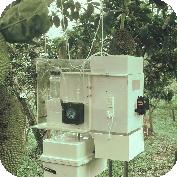
\includegraphics[width = 0.89\textwidth] {pics/trap.pdf}
        \captionof{figure}[Trap set up at the jackfruit orchard.]{}
        \label{fig:case3Pic}
    \end{center}
\end{minipage}

\end{document}
